\section{Methodik}
\label{sec:methodik}

Die vorliegende Bachelorarbeit beschäftigt sich mit der Dekodierung verschiedener Dreiecksnetze mittels des Kodierungsstandards Brotli-G.
Diese Sektion dient dazu, einen detaillierten Einblick auf die Durchführung und Analyse des Experiments zu geben.
Das Experiment zielt darauf ab, komprimierte Dreiecksnetze auf der GPU zu dekomprimieren.
Insbesondere sollen das Kompressionsverhältnis, die Dekompressionsgeschwindigkeit und die visuelle Qualität quantitativ ausgewertet werden. \newline

In diesem Abschnitt folgt eine kleine Beschreibung, wie die Kompressionspipeline aussieht.
In den folgenden Kapiteln werden die einzelnen Teilschritte genauer erläutert. \newline
Zu Beginn muss der Datensatz mittels Brotli-G kodiert werden.
Der Einfachheit halber wird in diesem Abschnitt von einem einzigen Dreiecksnetz gesprochen.
Der Meshoptimizer von Zeux \cite{Zeux} ist dafür verantwortlich, aus den Positionen und Indizes die Daten für die Meshlets zu generieren.
Dazu wurde ein Binärformat entworfen, welches die relevanten Daten zum Darstellen des gesamten Dreiecksnetzes speichert.
Das Binärformat besteht dementsprechend aus dem Meshlet Descriptor, Vertex Ressourcen (Positionen und Normalen) und den Indizes zur Generierung von Primitiven. \newline
Dieses Binärformat wird als Gesamtes komprimiert.
Anschließend werden die GPU-Ressourcen für die Eingabe (komprimiertes Dreiecksnetz) und Ausgabe (dekomprimiertes Dreiecksnetz) angelegt. \newline
Für die Ausgabe wird eine \glqq Unordered Access View (UAV)\grqq\ verwendet.
Wie der Name schon vermuten lässt, bietet diese eine flexiblere Möglichkeit, gleichzeitig an verschiedenen Orten zu lesen und zu schreiben.
Besonders von Vorteil ist dieser Ressourcentyp für die parallele Verarbeitung.
So können einzelne Threads von der Ressource lesen/schreiben, ohne warten zu müssen, bis ein anderer Thread die Ressource wieder freigibt \cite{Microsoft2021}. \newline
Die UAV wird im Compute Shader als Output Buffer gesetzt, und mit den dekomprimierten Daten des Dreiecksnetzes gefüllt.

Abschließend wird die UAV im Mesh Shader gesetzt und die Meshlets und somit das gesamte Dreiecksnetz werden aus den Binärdaten rekonstruiert. \newline
Der gesamte Vorgang ist in Abbildung~\ref{fig:projekt} zu sehen.

\begin{figure}[htb]
  \centering  
  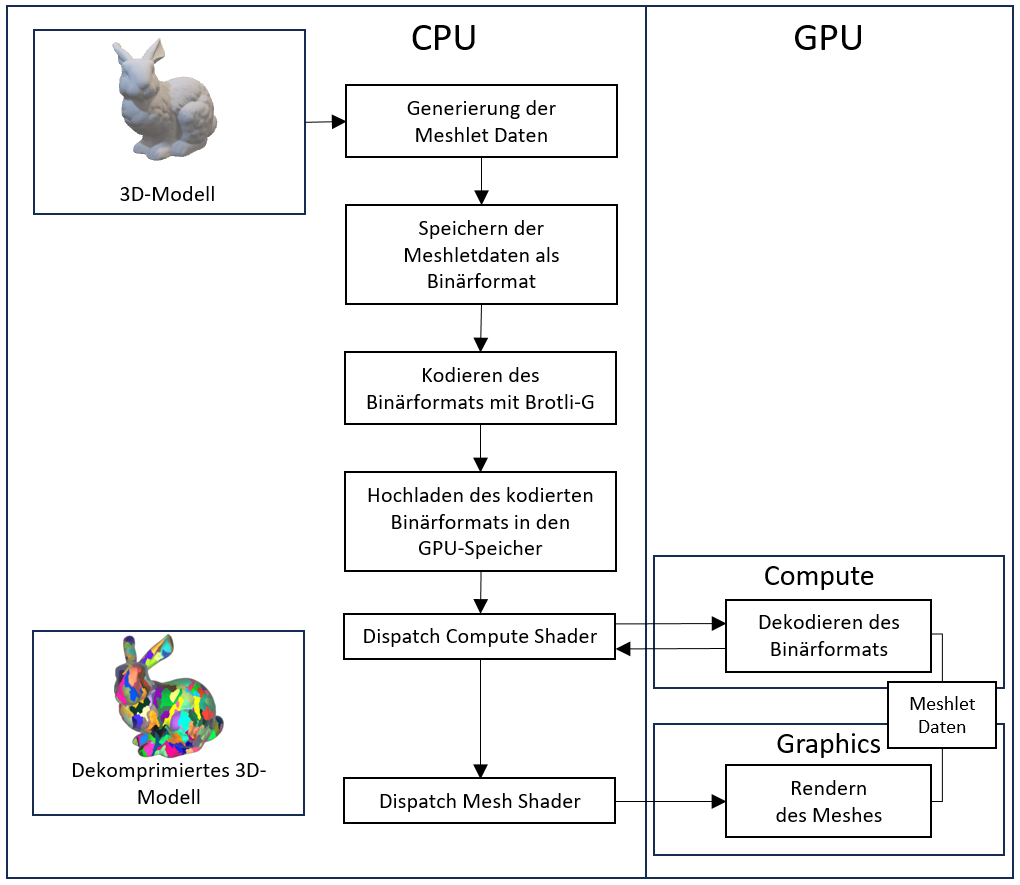
\includegraphics[scale=0.58]{Bilder/Ablauf_Projekt.png}
  \caption[Flussdiagramm des Ablaufs]{\textbf{Flussdiagramm des Ablaufs} Abbildung der Dekompressionspipeline.}
  \label{fig:projekt}
\end{figure}

Nach diesem Schritt könnten die Daten der UAV von der CPU ausgelesen werden.
Mit den Daten können StructuredBuffer gefüllt werden, welche die Daten der Meshlets erhalten.
Dieser Schritt ist jedoch als unnötig anzusehen, wenn nicht noch zusätzliche Informationen mit dem dekomprimierten Dreiecksnetz berechnet werden müssen.
Der Output Buffer des Brotli-G Dekodierers beinhaltet die benötigten Meshlet Daten, um das Dreiecksnetz zu rekonstruieren.
So kann ein GPU-Buffer außerhalb der Brotli-G Klasse angelegt werden, den Brotli-G als Output Buffer verwendet.
Dieser Buffer und dessen Daten werden nach dem Destruktor von Brotli-Gs Dekodierer nicht freigegeben.
Dadurch wird dieser Buffer nicht freigegeben, nachdem der Dekompressionsschritt von Brotli-G abgeschlossen ist.
Somit kann der Mesh Shader direkt auf die Daten zugreifen, die nach dem Dekodieren noch im GPU-RAM liegen.
Abschließend wird dem Mesh Shader die Speicheradresse des Output Daten Buffer übergeben, aus dem das Dreiecksnetz rekonstruiert werden kann.